
\documentclass[serif]{beamer}
\usepackage{float}
\usepackage{tikz}
\usepackage{amssymb}
\usepackage{amsmath}
\usepackage{mathtools}
\usepackage{pgfplots}
\usepackage{multirow}
\usepackage{caption}
\captionsetup[figure]{labelformat=empty}
\usetikzlibrary{fit,decorations.pathreplacing,snakes,arrows,shapes,automata, backgrounds,calc,shadings,shapes.arrows,shapes.symbols,shadows}
\usetikzlibrary{patterns} 

\setbeamertemplate{caption}[numbered]
\setbeamertemplate{navigation symbols}{} 
\setbeamertemplate{footline}[page number]

%***************************************************************************************
%********************STUFF FOR DRAWING NETWORK DIAGRAM *********************************


\makeatletter
\pgfkeys{/pgf/.cd,
  parallelepiped offset x/.initial=2mm,
  parallelepiped offset y/.initial=2mm
}
\pgfdeclareshape{parallelepiped}
{
  \inheritsavedanchors[from=rectangle] % this is nearly a rectangle
  \inheritanchorborder[from=rectangle]
  \inheritanchor[from=rectangle]{north}
  \inheritanchor[from=rectangle]{north west}
  \inheritanchor[from=rectangle]{north east}
  \inheritanchor[from=rectangle]{center}
  \inheritanchor[from=rectangle]{west}
  \inheritanchor[from=rectangle]{east}
  \inheritanchor[from=rectangle]{mid}
  \inheritanchor[from=rectangle]{mid west}
  \inheritanchor[from=rectangle]{mid east}
  \inheritanchor[from=rectangle]{base}
  \inheritanchor[from=rectangle]{base west}
  \inheritanchor[from=rectangle]{base east}
  \inheritanchor[from=rectangle]{south}
  \inheritanchor[from=rectangle]{south west}
  \inheritanchor[from=rectangle]{south east}
  \backgroundpath{
    % store lower right in xa/ya and upper right in xb/yb
    \southwest \pgf@xa=\pgf@x \pgf@ya=\pgf@y
    \northeast \pgf@xb=\pgf@x \pgf@yb=\pgf@y
    \pgfmathsetlength\pgfutil@tempdima{\pgfkeysvalueof{/pgf/parallelepiped
      offset x}}
    \pgfmathsetlength\pgfutil@tempdimb{\pgfkeysvalueof{/pgf/parallelepiped
      offset y}}
    \def\ppd@offset{\pgfpoint{\pgfutil@tempdima}{\pgfutil@tempdimb}}
    \pgfpathmoveto{\pgfqpoint{\pgf@xa}{\pgf@ya}}
    \pgfpathlineto{\pgfqpoint{\pgf@xb}{\pgf@ya}}
    \pgfpathlineto{\pgfqpoint{\pgf@xb}{\pgf@yb}}
    \pgfpathlineto{\pgfqpoint{\pgf@xa}{\pgf@yb}}
    \pgfpathclose
    \pgfpathmoveto{\pgfqpoint{\pgf@xb}{\pgf@ya}}
    \pgfpathlineto{\pgfpointadd{\pgfpoint{\pgf@xb}{\pgf@ya}}{\ppd@offset}}
    \pgfpathlineto{\pgfpointadd{\pgfpoint{\pgf@xb}{\pgf@yb}}{\ppd@offset}}
    \pgfpathlineto{\pgfpointadd{\pgfpoint{\pgf@xa}{\pgf@yb}}{\ppd@offset}}
    \pgfpathlineto{\pgfqpoint{\pgf@xa}{\pgf@yb}}
    \pgfpathmoveto{\pgfqpoint{\pgf@xb}{\pgf@yb}}
    \pgfpathlineto{\pgfpointadd{\pgfpoint{\pgf@xb}{\pgf@yb}}{\ppd@offset}}
  }
}
\makeatother

\tikzset{l3 switch/.style={
    parallelepiped,fill=switch, draw=white,
    minimum width=0.75cm,
    minimum height=0.75cm,
    parallelepiped offset x=1.75mm,
    parallelepiped offset y=1.25mm,
    path picture={
      \node[fill=white,
        circle,
        minimum size=6pt,
        inner sep=0pt,
        append after command={
          \pgfextra{
            \foreach \angle in {0,45,...,360}
            \draw[-latex,fill=white] (\tikzlastnode.\angle)--++(\angle:2.25mm);
          }
        }
      ] 
       at ([xshift=-0.75mm,yshift=-0.5mm]path picture bounding box.center){};
    }
  },
  ports/.style={
    line width=0.3pt,
    top color=gray!20,
    bottom color=gray!80
  },
  rack switch/.style={
    parallelepiped,fill=white, draw,
    minimum width=1.25cm,
    minimum height=0.25cm,
    parallelepiped offset x=2mm,
    parallelepiped offset y=1.25mm,
    xscale=-1,
    path picture={
      \draw[top color=gray!5,bottom color=gray!40]
      (path picture bounding box.south west) rectangle 
      (path picture bounding box.north east);
      \coordinate (A-west) at ([xshift=-0.2cm]path picture bounding box.west);
      \coordinate (A-center) at ($(path picture bounding box.center)!0!(path
        picture bounding box.south)$);
      \foreach \x in {0.275,0.525,0.775}{
        \draw[ports]([yshift=-0.05cm]$(A-west)!\x!(A-center)$)
          rectangle +(0.1,0.05);
        \draw[ports]([yshift=-0.125cm]$(A-west)!\x!(A-center)$)
          rectangle +(0.1,0.05);
       } 
      \coordinate (A-east) at (path picture bounding box.east);
      \foreach \x in {0.085,0.21,0.335,0.455,0.635,0.755,0.875,1}{
        \draw[ports]([yshift=-0.1125cm]$(A-east)!\x!(A-center)$)
          rectangle +(0.05,0.1);       
      }
    }
  },
  server/.style={
    parallelepiped,
    fill=white, draw,
    minimum width=0.35cm,
    minimum height=0.75cm,
    parallelepiped offset x=3mm,
    parallelepiped offset y=2mm,
    xscale=-1,
    path picture={
      \draw[top color=gray!5,bottom color=gray!40]
      (path picture bounding box.south west) rectangle 
      (path picture bounding box.north east);
      \coordinate (A-center) at ($(path picture bounding box.center)!0!(path
        picture bounding box.south)$);
      \coordinate (A-west) at ([xshift=-0.575cm]path picture bounding box.west);
      \draw[ports]([yshift=0.1cm]$(A-west)!0!(A-center)$)
        rectangle +(0.2,0.065);
      \draw[ports]([yshift=0.01cm]$(A-west)!0.085!(A-center)$)
        rectangle +(0.15,0.05);
      \fill[black]([yshift=-0.35cm]$(A-west)!-0.1!(A-center)$)
        rectangle +(0.235,0.0175);
      \fill[black]([yshift=-0.385cm]$(A-west)!-0.1!(A-center)$)
        rectangle +(0.235,0.0175);
      \fill[black]([yshift=-0.42cm]$(A-west)!-0.1!(A-center)$)
        rectangle +(0.235,0.0175);
    }  
  },
}

% Styles for interfaces and edge labels
\tikzset{%
  interface/.style={draw, rectangle, rounded corners, font=\LARGE\sffamily},
  ethernet/.style={interface, fill=yellow!50},% ethernet interface
  serial/.style={interface, fill=green!70},% serial interface
  speed/.style={sloped, anchor=south, font=\large\sffamily},% line speed at edge
  route/.style={draw, shape=single arrow, single arrow head extend=4mm,
    minimum height=1.7cm, minimum width=3mm, white, fill=switch!20,
    drop shadow={opacity=.8, fill=switch}, font=\tiny}% inroute/outroute arrows
}
\newcommand*{\shift}{1.3cm}% For placing the arrows later

\makeatletter
\pgfdeclareradialshading[tikz@ball]{cloud}{\pgfpoint{-0.275cm}{0.4cm}}{%
  color(0cm)=(tikz@ball!75!white);
  color(0.1cm)=(tikz@ball!85!white); 
  color(0.2cm)=(tikz@ball!95!white); 
  color(0.7cm)=(tikz@ball!89!black); 
  color(1cm)=(tikz@ball!75!black)
}
\tikzoption{cloud color}{\pgfutil@colorlet{tikz@ball}{#1}%
  \def\tikz@shading{cloud}\tikz@addmode{\tikz@mode@shadetrue}}
\makeatother

\tikzset{my cloud/.style={
     cloud, draw, aspect=2,
     cloud color={gray!5!white}
  }
}

%***************************************************************************************
%***************************************************************************************
 

\begin{document}
\title{\centering \textbf{Verification of Fault-Tolerant Clock\\
Synchronization Algorithms\\ (Benchmark Proposal)}} 
\author{\textcolor{red}{Sergiy Bogomolov$^{1}$, Christian Herrera$^{2}$ and Wilfried Steiner$^{3}$}  
	\center{IST Austria$^{1}$, \\University of Freiburg$^{2}$, \\TTTech Computertechnik AG$^{3}$ }}
\date{April 11th, 2016}
\begin{frame}
\titlepage
\end{frame}
 

\begin{frame}\frametitle{\textbf{Motivation -- TTEthernet}}
\emph{\textcolor{blue}{TTEthernet}}  
\begin{itemize}
\item implementation of the \emph{\textcolor{blue}{Ethernet}} standard which complies with
\textcolor{red}{time-critical}, \textcolor{red}{deterministic} and \textcolor{red}{safety-critical} real-time requirements.

\item[] \textcolor{white}{used in commercial \textcolor{white}{hardware} and \textcolor{white}{software} products,
e.g. the avionics of the \emph{\textcolor{white}{Orion Space Program}}.}

\item[] \textcolor{white}{assumes a \textcolor{white}{global time base} for tolerating faulty behavior of safety critical systems.}
	\begin{itemize}
		\item[]  \textcolor{white}{any two logical clocks of two distributed
						components must read \textcolor{white}{the same values} at any time (\emph{\textcolor{white}{precision}}).
						The precision is ensured by a \textcolor{white}{clock synchronization algorithm}. }
	\end{itemize}
\end{itemize}
\end{frame} 

\begin{frame}\frametitle{\textbf{Motivation -- TTEthernet}}
\emph{\textcolor{blue}{TTEthernet}}  
\begin{itemize}
\item implementation of the \emph{\textcolor{blue}{Ethernet}} standard which complies with
\textcolor{red}{time-critical}, \textcolor{red}{deterministic} and \textcolor{red}{safety-critical} real-time requirements.

\item used in commercial \textcolor{red}{hardware} and \textcolor{red}{software} products,
e.g. the avionics of the \emph{\textcolor{blue}{Orion Space Program}}.

\item[] \textcolor{white}{assumes a \textcolor{white}{global time base} for tolerating faulty behavior of safety critical systems.}
	\begin{itemize}
		\item[]  \textcolor{white}{any two logical clocks of two distributed
						components must read \textcolor{white}{the same values} at any time (\emph{\textcolor{white}{precision}}).
						The precision is ensured by a \textcolor{white}{clock synchronization algorithm}. }
	\end{itemize}
\end{itemize}
\end{frame} 


\begin{frame}\frametitle{\textbf{Motivation -- TTEthernet}}
\emph{\textcolor{blue}{TTEthernet}}  
\begin{itemize}
\item implementation of the \emph{\textcolor{blue}{Ethernet}} standard which complies with
\textcolor{red}{time-critical}, \textcolor{red}{deterministic} and \textcolor{red}{safety-critical} real-time requirements.

\item used in commercial \textcolor{red}{hardware} and \textcolor{red}{software} products,
e.g. the avionics of the \emph{\textcolor{blue}{Orion Space Program}}.

\item assumes a \textcolor{red}{global time base} for tolerating faulty behavior of safety critical systems, i.e.
	\begin{itemize}
		\item  \textcolor{red}{any two logical clocks} of two
						components must read \textcolor{red}{the same values} at any time (\emph{\textcolor{blue}{precision}}). 
						The precision is ensured by a \textcolor{blue}{clock synchronization algorithm}.
	\end{itemize}
\end{itemize}
\end{frame} 
 
\begin{frame}\frametitle{\textbf{Our Goal}}
We propose a \emph{\textcolor{blue}{benchmark}} which can be used as a basis for: 
\begin{itemize}
	\item verifying the \emph{\textcolor{blue}{precision}} of the clock synchronization algorithm. 
	\item implementing optimization techniques for verification purposes, e.g. 
				\textcolor{red}{detection} and \textcolor{red}{reduction} of \emph{\textcolor{blue}{quasi-dependent variables}}.
	\item verifying other clock synchronization algorithms, e.g. \emph{\textcolor{blue}{interactive convergence algorithm}}	and 
				\emph{\textcolor{blue}{byzantine clock synchronization}}.
\end{itemize}
\end{frame}


\begin{frame}\frametitle{\textbf{Fault-Tolerant Configuration}}
\centering
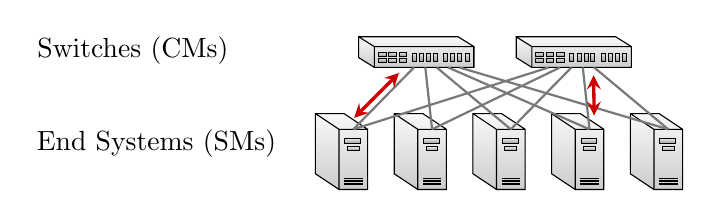
\begin{tikzpicture}

\node[server](server 1){};
\node[server, right of= server 1](server 2){};
\node[server, right of= server 2](server 3){};

\node[rack switch, above of=server 2,xshift=0.1cm,yshift=0.3cm]
  (rack switch 1){};
%lineas conectando un CM con un SM
\draw[thick,darkgray!10!gray] (server 1.north)--(rack switch 1);
\draw[thick,darkgray!10!gray] (server 2.north)--(rack switch 1);
\draw[thick,darkgray!10!gray] (server 3.north)--(rack switch 1);


\begin{scope}[xshift=3.5cm]
  \node[server, right of= server 3](server 5){};
  \node[server, right of= server 5](server 6){};

  \node[rack switch, above of=server 5,xshift=0.1cm,yshift=0.3cm]
  (rack switch 2){};
  \draw[thick,darkgray!10!gray] (server 5.north)--(rack switch 1);
  \draw[thick,darkgray!10!gray] (server 6.north)--(rack switch 1);
  \draw[thick,darkgray!10!gray] (server 5.north)--(rack switch 2);
  \draw[thick,darkgray!10!gray] (server 6.north)--(rack switch 2);
  \draw[thick,darkgray!10!gray] (server 1.north)--(rack switch 2);
	\draw[thick,darkgray!10!gray] (server 2.north)--(rack switch 2);
	\draw[thick,darkgray!10!gray] (server 3.north)--(rack switch 2);
  
\end{scope}
 
 
 

% = = = = = = = = = = = = = = = =
% Labels
% = = = = = = = = = = = = = = = =


\node[xshift=-3.5cm,yshift=0.2cm,left of = server 3,align=left](lev1)
  {End Systems (SMs)};

\node[xshift=-0.3cm,yshift=0.18cm,above of = lev1,align=left](lev2)
  {Switches (CMs)};



% = = = = = = = = = = = = = = = =
% paths
% = = = = = = = = = = = = = = = =
 

\draw[stealth-stealth,very thick, red!80!black,shorten <=0.1cm, shorten >=0.1cm]
  ([xshift=-0.25cm]rack switch 2.south)--
  ([yshift=0.075cm,xshift=-0.06cm]server 6.north);
 
 \draw[stealth-stealth,very thick, red!80!black,shorten <=0.1cm, shorten >=0.1cm]
  ([xshift=0.15cm]rack switch 1.south)--
  ([yshift=0.075cm,xshift=0.06cm]server 2.north);

\end{tikzpicture}
\begin{enumerate}
	\item[] \textcolor{white}{SMs send the current value of their clocks to each CM. Then each CM obtains 
				the \textcolor{white}{median} of the values sent by all SMs.} 
	\item[] \textcolor{white}{CMs send the mentioned result to each SM. Then each SM 
				updates its clock by using the \textcolor{white}{median} of the values sent by all CMs.} 			
\end{enumerate}
\end{frame}

 
\begin{frame}\frametitle{\textbf{TTEthernet's Clock Synchronization Algorithm}}
\centering
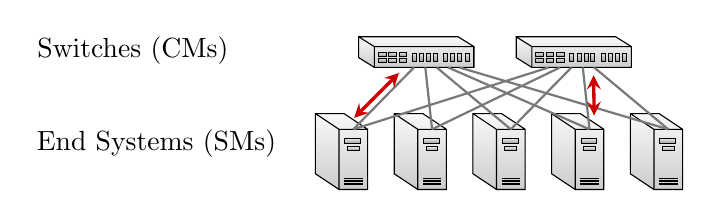
\begin{tikzpicture}

\node[server](server 1){};
\node[server, right of= server 1](server 2){};
\node[server, right of= server 2](server 3){};

\node[rack switch, above of=server 2,xshift=0.1cm,yshift=0.3cm]
  (rack switch 1){};
%lineas conectando un CM con un SM
\draw[thick,darkgray!10!gray] (server 1.north)--(rack switch 1);
\draw[thick,darkgray!10!gray] (server 2.north)--(rack switch 1);
\draw[thick,darkgray!10!gray] (server 3.north)--(rack switch 1);


\begin{scope}[xshift=3.5cm]
  \node[server, right of= server 3](server 5){};
  \node[server, right of= server 5](server 6){};

  \node[rack switch, above of=server 5,xshift=0.1cm,yshift=0.3cm]
  (rack switch 2){};
  \draw[thick,darkgray!10!gray] (server 5.north)--(rack switch 1);
  \draw[thick,darkgray!10!gray] (server 6.north)--(rack switch 1);
  \draw[thick,darkgray!10!gray] (server 5.north)--(rack switch 2);
  \draw[thick,darkgray!10!gray] (server 6.north)--(rack switch 2);
  \draw[thick,darkgray!10!gray] (server 1.north)--(rack switch 2);
	\draw[thick,darkgray!10!gray] (server 2.north)--(rack switch 2);
	\draw[thick,darkgray!10!gray] (server 3.north)--(rack switch 2);
  
\end{scope}
 
 
 

% = = = = = = = = = = = = = = = =
% Labels
% = = = = = = = = = = = = = = = =


\node[xshift=-3.5cm,yshift=0.2cm,left of = server 3,align=left](lev1)
  {End Systems (SMs)};

\node[xshift=-0.3cm,yshift=0.18cm,above of = lev1,align=left](lev2)
  {Switches (CMs)};



% = = = = = = = = = = = = = = = =
% paths
% = = = = = = = = = = = = = = = =
 

\draw[stealth-stealth,very thick, red!80!black,shorten <=0.1cm, shorten >=0.1cm]
  ([xshift=-0.25cm]rack switch 2.south)--
  ([yshift=0.075cm,xshift=-0.06cm]server 6.north);
 
 \draw[stealth-stealth,very thick, red!80!black,shorten <=0.1cm, shorten >=0.1cm]
  ([xshift=0.15cm]rack switch 1.south)--
  ([yshift=0.075cm,xshift=0.06cm]server 2.north);

\end{tikzpicture}
\begin{enumerate}
	\item SMs send the current value of their clocks to each CM. Then each CM obtains 
				the \textcolor{red}{median} of the values sent by all SMs. 
	\item[] \textcolor{white}{CMs send the mentioned result to each SM. Then each SM 
				updates its clock by using the \textcolor{white}{median} of the values sent by all CMs.} 			
\end{enumerate}
\end{frame}

\begin{frame}\frametitle{\textbf{TTEthernet's Clock Synchronization Algorithm}}
\centering
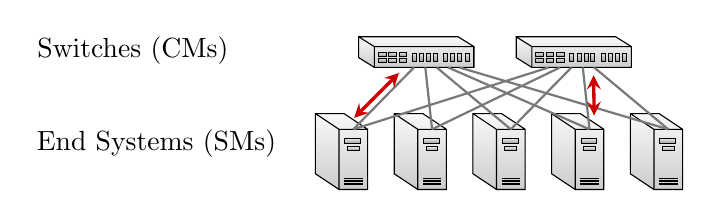
\begin{tikzpicture}

\node[server](server 1){};
\node[server, right of= server 1](server 2){};
\node[server, right of= server 2](server 3){};

\node[rack switch, above of=server 2,xshift=0.1cm,yshift=0.3cm]
  (rack switch 1){};
%lineas conectando un CM con un SM
\draw[thick,darkgray!10!gray] (server 1.north)--(rack switch 1);
\draw[thick,darkgray!10!gray] (server 2.north)--(rack switch 1);
\draw[thick,darkgray!10!gray] (server 3.north)--(rack switch 1);


\begin{scope}[xshift=3.5cm]
  \node[server, right of= server 3](server 5){};
  \node[server, right of= server 5](server 6){};

  \node[rack switch, above of=server 5,xshift=0.1cm,yshift=0.3cm]
  (rack switch 2){};
  \draw[thick,darkgray!10!gray] (server 5.north)--(rack switch 1);
  \draw[thick,darkgray!10!gray] (server 6.north)--(rack switch 1);
  \draw[thick,darkgray!10!gray] (server 5.north)--(rack switch 2);
  \draw[thick,darkgray!10!gray] (server 6.north)--(rack switch 2);
  \draw[thick,darkgray!10!gray] (server 1.north)--(rack switch 2);
	\draw[thick,darkgray!10!gray] (server 2.north)--(rack switch 2);
	\draw[thick,darkgray!10!gray] (server 3.north)--(rack switch 2);
  
\end{scope}
 
 
 

% = = = = = = = = = = = = = = = =
% Labels
% = = = = = = = = = = = = = = = =


\node[xshift=-3.5cm,yshift=0.2cm,left of = server 3,align=left](lev1)
  {End Systems (SMs)};

\node[xshift=-0.3cm,yshift=0.18cm,above of = lev1,align=left](lev2)
  {Switches (CMs)};



% = = = = = = = = = = = = = = = =
% paths
% = = = = = = = = = = = = = = = =
 

\draw[stealth-stealth,very thick, red!80!black,shorten <=0.1cm, shorten >=0.1cm]
  ([xshift=-0.25cm]rack switch 2.south)--
  ([yshift=0.075cm,xshift=-0.06cm]server 6.north);
 
 \draw[stealth-stealth,very thick, red!80!black,shorten <=0.1cm, shorten >=0.1cm]
  ([xshift=0.15cm]rack switch 1.south)--
  ([yshift=0.075cm,xshift=0.06cm]server 2.north);

\end{tikzpicture}
\begin{enumerate}
	\item SMs send the current value of their clocks to each CM. Then each CM obtains 
				the \textcolor{red}{median} of the values sent by all SMs. 
	\item CMs send the mentioned result to each SM. Then each SM 
				updates its clock by using the \textcolor{red}{median} of the values sent by all CMs. 	
\end{enumerate}
\end{frame}
 

\begin{frame}\frametitle{\textbf{Benchmark -- Network of Hybrid Automata $\mathcal{N}$}}
\centering
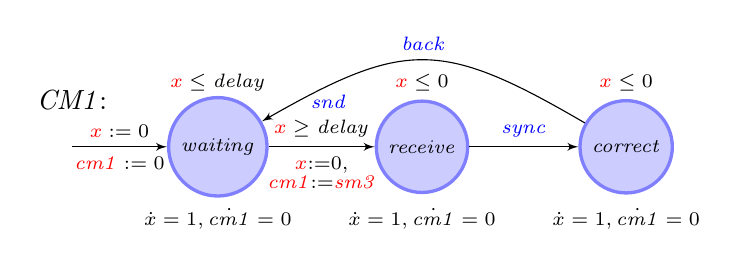
\begin{tikzpicture}[>=latex',join=bevel, scale=0.7]
 \tikzstyle{every state}=     [draw=blue!50,very thick,fill=blue!20]
 \coordinate (init) at (-110bp,77bp);
 \node (A) at (-35bp,77bp) [state] {\scriptsize$\mathit{waiting}$};
 \node (B) at (70bp,77bp) [state] {\scriptsize$\mathit{receive}$};
 \node (C) at (175bp,77bp) [state] {\scriptsize$\mathit{correct}$};
  \node (D) at (22bp,100bp) [] {\scriptsize$\mathit{\textcolor{blue}{snd}}$};

 \node (Asubscript) at (-35bp, 40bp)  {\scriptsize $\dot{x} = 1, \dot{\mathit{cm1}} = 0$};
 \node (Asuperscript) at (-35bp, 110bp)  {\scriptsize $\textcolor{red}{x} \le \mathit{delay}$}; %vertical diff is 24bp
 \node (Bsubscript) at (70bp, 40bp) {\scriptsize $\dot{x} = 1, \dot{\mathit{cm1}} = 0$}; %horizontal diff is 105bp
 \node (Bsuperscript) at (70bp, 110bp)  {\scriptsize $\textcolor{red}{x} \le 0$}; 
 \node (Csubscript) at (175bp, 40bp) {\scriptsize $\dot{x} = 1, \dot{\mathit{cm1}} = 0$}; 
 \node (Csuperscript) at (175bp, 110bp)  {\scriptsize $\textcolor{red}{x} \le 0$};

 \node (automatonname) at (-110bp, 101bp)  {$\mathit{CM1}$:};


 \draw [->] (init) to node[above] {\scriptsize $\textcolor{red}{x} := 0$} node[below] 
 						{\scriptsize $\mathit{\textcolor{red}{cm1}} := 0$}(A);
 \draw [->] (A) to node[above] {\scriptsize $\textcolor{red}{x} \geq \mathit{delay}$} node[below]
 		{ $\substack{\textcolor{red}{x}:=0,\\ \mathit{\textcolor{red}{cm1}}:= \mathit{\textcolor{red}{sm3}}}$}(B);
 \draw [->] (B) to node[above] {\scriptsize$\mathit{\textcolor{blue}{sync}}$} (C);
 \draw [->] (C) to[distance=3cm, bend right]  node[above] {\scriptsize$\mathit{\textcolor{blue}{back}}$} (A);

\end{tikzpicture}

\begin{tikzpicture}[>=latex',join=bevel,scale=0.7]
 \tikzstyle{every state}=     [draw=white,very thick,fill=white]
 \coordinate (init) at (-105bp,77bp);
 \node (A) at (-35bp,77bp) [state] {\scriptsize$\mathit{\textcolor{white}{work}}$};
 \node (B) at (70bp,77bp) [state] {\scriptsize$\mathit{\textcolor{white}{send}}$};
 \node (C) at (190bp,77bp) [state] {\scriptsize$\mathit{\textcolor{white}{sync}}$};

 \node (Asubscript) at (-35bp, 46bp)  {\scriptsize $\textcolor{white}{\dot{\mathit{sm3= 1}}} $};
 \node (Bsubscript) at (70bp, 46bp) {\scriptsize $\textcolor{white}{\dot{\mathit{sm3 = 1}}}$}; %horizontal diff is 105bp
 \node (Csubscript) at (190bp, 46bp) {\scriptsize $\textcolor{white}{\dot{\mathit{sm3 = 1}}}$}; 

 \node (automatonname) at (-110bp, 101bp)  {$\mathit{\textcolor{white}{SM3:}}$};


 \draw [->,white] (init) to node[above] {\scriptsize $\mathit{\textcolor{white}{sm3:=0}}$} (A);
 \draw [->,white] (A) to node[above] {\scriptsize $\mathit{\textcolor{white}{snd}}$} 
 				node[below]{$\substack{\mathit{\textcolor{white}{sm3}}:=\\ \mathit{\textcolor{white}{sm3}+\mathit{drift3}}}$}(B);
 \draw [->,white] (B) to node[above] {\scriptsize $\mathit{\textcolor{white}{sync}}$} 
 					node[below]{$\substack{\mathit{\textcolor{white}{sm3}}:= \\ 
 						(\mathit{\textcolor{white}{cm1}}+\mathit{\textcolor{white}{cm2}})/2}$}(C);
 	 \draw [->,white] (C) to[bend right]  node[above] {\scriptsize$\mathit{\textcolor{white}{back}}$} (A);				
\end{tikzpicture}

\emph{\textcolor{white}{Precision: $\forall i\neq j\in\mathbb{N}\bullet \ sm_i > sm_j \implies sm_i-sm_j \leq 2*\mathit{maxdrift}$}} 
\end{frame}


\begin{frame}\frametitle{\textbf{Benchmark -- Network of Hybrid Automata $\mathcal{N}$}}
\centering
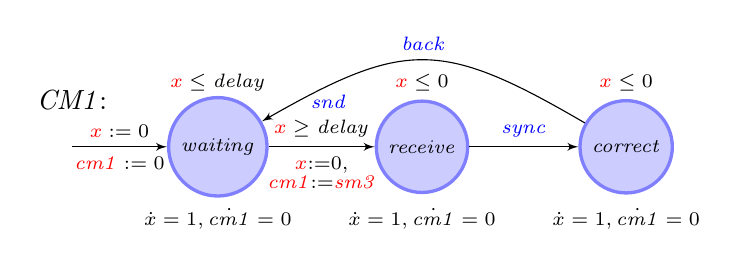
\begin{tikzpicture}[>=latex',join=bevel, scale=0.7]
 \tikzstyle{every state}=     [draw=blue!50,very thick,fill=blue!20]
 \coordinate (init) at (-110bp,77bp);
 \node (A) at (-35bp,77bp) [state] {\scriptsize$\mathit{waiting}$};
 \node (B) at (70bp,77bp) [state] {\scriptsize$\mathit{receive}$};
 \node (C) at (175bp,77bp) [state] {\scriptsize$\mathit{correct}$};
  \node (D) at (22bp,100bp) [] {\scriptsize$\mathit{\textcolor{blue}{snd}}$};

 \node (Asubscript) at (-35bp, 40bp)  {\scriptsize $\dot{x} = 1, \dot{\mathit{cm1}} = 0$};
 \node (Asuperscript) at (-35bp, 110bp)  {\scriptsize $\textcolor{red}{x} \le \mathit{delay}$}; %vertical diff is 24bp
 \node (Bsubscript) at (70bp, 40bp) {\scriptsize $\dot{x} = 1, \dot{\mathit{cm1}} = 0$}; %horizontal diff is 105bp
 \node (Bsuperscript) at (70bp, 110bp)  {\scriptsize $\textcolor{red}{x} \le 0$}; 
 \node (Csubscript) at (175bp, 40bp) {\scriptsize $\dot{x} = 1, \dot{\mathit{cm1}} = 0$}; 
 \node (Csuperscript) at (175bp, 110bp)  {\scriptsize $\textcolor{red}{x} \le 0$};

 \node (automatonname) at (-110bp, 101bp)  {$\mathit{CM1}$:};


 \draw [->] (init) to node[above] {\scriptsize $\textcolor{red}{x} := 0$} node[below] 
 						{\scriptsize $\mathit{\textcolor{red}{cm1}} := 0$}(A);
 \draw [->] (A) to node[above] {\scriptsize $\textcolor{red}{x} \geq \mathit{delay}$} node[below]
 		{ $\substack{\textcolor{red}{x}:=0,\\ \mathit{\textcolor{red}{cm1}}:= \mathit{\textcolor{red}{sm3}}}$}(B);
 \draw [->] (B) to node[above] {\scriptsize$\mathit{\textcolor{blue}{sync}}$} (C);
 \draw [->] (C) to[distance=3cm, bend right]  node[above] {\scriptsize$\mathit{\textcolor{blue}{back}}$} (A);

\end{tikzpicture}

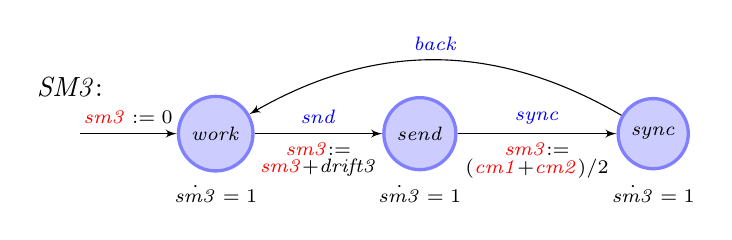
\begin{tikzpicture}[>=latex',join=bevel,scale=0.7]
 \tikzstyle{every state}=     [draw=blue!50,very thick,fill=blue!20]
 \coordinate (init) at (-105bp,77bp);
 \node (A) at (-35bp,77bp) [state] {\scriptsize$\mathit{work}$};
 \node (B) at (70bp,77bp) [state] {\scriptsize$\mathit{send}$};
 \node (C) at (190bp,77bp) [state] {\scriptsize$\mathit{sync}$};

 \node (Asubscript) at (-35bp, 46bp)  {\scriptsize $\dot{\mathit{sm3}} = 1$};
 \node (Bsubscript) at (70bp, 46bp) {\scriptsize $\dot{\mathit{sm3}} = 1$}; %horizontal diff is 105bp
 \node (Csubscript) at (190bp, 46bp) {\scriptsize $\dot{\mathit{sm3}} = 1$}; 

 \node (automatonname) at (-110bp, 101bp)  {$\mathit{SM3}$:};


 \draw [->] (init) to node[above] {\scriptsize $\mathit{\textcolor{red}{sm3}}:=0$} (A);
 \draw [->] (A) to node[above] {\scriptsize $\mathit{\textcolor{blue}{snd}}$} 
 				node[below]{$\substack{\mathit{\textcolor{red}{sm3}}:=\\ \mathit{\textcolor{red}{sm3}}+\mathit{drift3}}$}(B);
 \draw [->] (B) to node[above] {\scriptsize $\mathit{\textcolor{blue}{sync}}$} 
 					node[below]{$\substack{\mathit{\textcolor{red}{sm3}}:= \\ 
 						(\mathit{\textcolor{red}{cm1}}+\mathit{\textcolor{red}{cm2}})/2}$}(C);
 	 \draw [->] (C) to[bend right]  node[above] {\scriptsize$\mathit{\textcolor{blue}{back}}$} (A);				
\end{tikzpicture}

\emph{\textcolor{white}{Precision: $\forall i\neq j\in\mathbb{N}\bullet \ sm_i > sm_j \implies sm_i-sm_j \leq 2*\mathit{maxdrift}$}} 
\end{frame}


\begin{frame}\frametitle{\textbf{Benchmark -- Network of Hybrid Automata $\mathcal{N}$}}
\centering
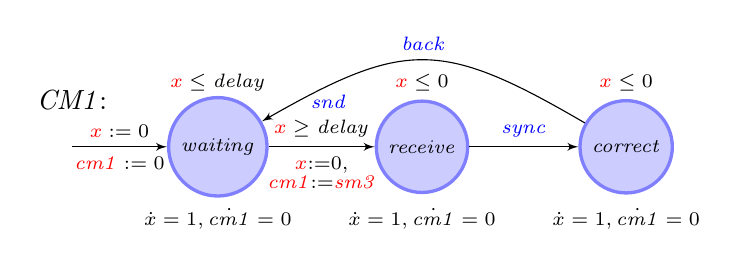
\begin{tikzpicture}[>=latex',join=bevel, scale=0.7]
 \tikzstyle{every state}=     [draw=blue!50,very thick,fill=blue!20]
 \coordinate (init) at (-110bp,77bp);
 \node (A) at (-35bp,77bp) [state] {\scriptsize$\mathit{waiting}$};
 \node (B) at (70bp,77bp) [state] {\scriptsize$\mathit{receive}$};
 \node (C) at (175bp,77bp) [state] {\scriptsize$\mathit{correct}$};
  \node (D) at (22bp,100bp) [] {\scriptsize$\mathit{\textcolor{blue}{snd}}$};

 \node (Asubscript) at (-35bp, 40bp)  {\scriptsize $\dot{x} = 1, \dot{\mathit{cm1}} = 0$};
 \node (Asuperscript) at (-35bp, 110bp)  {\scriptsize $\textcolor{red}{x} \le \mathit{delay}$}; %vertical diff is 24bp
 \node (Bsubscript) at (70bp, 40bp) {\scriptsize $\dot{x} = 1, \dot{\mathit{cm1}} = 0$}; %horizontal diff is 105bp
 \node (Bsuperscript) at (70bp, 110bp)  {\scriptsize $\textcolor{red}{x} \le 0$}; 
 \node (Csubscript) at (175bp, 40bp) {\scriptsize $\dot{x} = 1, \dot{\mathit{cm1}} = 0$}; 
 \node (Csuperscript) at (175bp, 110bp)  {\scriptsize $\textcolor{red}{x} \le 0$};

 \node (automatonname) at (-110bp, 101bp)  {$\mathit{CM1}$:};


 \draw [->] (init) to node[above] {\scriptsize $\textcolor{red}{x} := 0$} node[below] 
 						{\scriptsize $\mathit{\textcolor{red}{cm1}} := 0$}(A);
 \draw [->] (A) to node[above] {\scriptsize $\textcolor{red}{x} \geq \mathit{delay}$} node[below]
 		{ $\substack{\textcolor{red}{x}:=0,\\ \mathit{\textcolor{red}{cm1}}:= \mathit{\textcolor{red}{sm3}}}$}(B);
 \draw [->] (B) to node[above] {\scriptsize$\mathit{\textcolor{blue}{sync}}$} (C);
 \draw [->] (C) to[distance=3cm, bend right]  node[above] {\scriptsize$\mathit{\textcolor{blue}{back}}$} (A);

\end{tikzpicture}

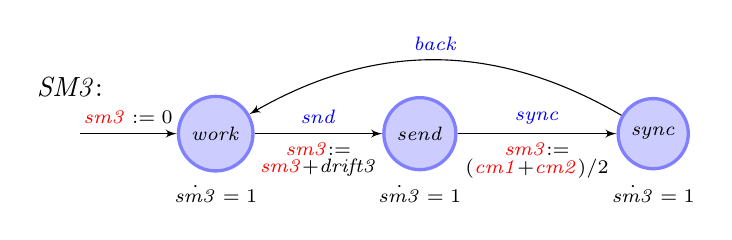
\begin{tikzpicture}[>=latex',join=bevel,scale=0.7]
 \tikzstyle{every state}=     [draw=blue!50,very thick,fill=blue!20]
 \coordinate (init) at (-105bp,77bp);
 \node (A) at (-35bp,77bp) [state] {\scriptsize$\mathit{work}$};
 \node (B) at (70bp,77bp) [state] {\scriptsize$\mathit{send}$};
 \node (C) at (190bp,77bp) [state] {\scriptsize$\mathit{sync}$};

 \node (Asubscript) at (-35bp, 46bp)  {\scriptsize $\dot{\mathit{sm3}} = 1$};
 \node (Bsubscript) at (70bp, 46bp) {\scriptsize $\dot{\mathit{sm3}} = 1$}; %horizontal diff is 105bp
 \node (Csubscript) at (190bp, 46bp) {\scriptsize $\dot{\mathit{sm3}} = 1$}; 

 \node (automatonname) at (-110bp, 101bp)  {$\mathit{SM3}$:};


 \draw [->] (init) to node[above] {\scriptsize $\mathit{\textcolor{red}{sm3}}:=0$} (A);
 \draw [->] (A) to node[above] {\scriptsize $\mathit{\textcolor{blue}{snd}}$} 
 				node[below]{$\substack{\mathit{\textcolor{red}{sm3}}:=\\ \mathit{\textcolor{red}{sm3}}+\mathit{drift3}}$}(B);
 \draw [->] (B) to node[above] {\scriptsize $\mathit{\textcolor{blue}{sync}}$} 
 					node[below]{$\substack{\mathit{\textcolor{red}{sm3}}:= \\ 
 						(\mathit{\textcolor{red}{cm1}}+\mathit{\textcolor{red}{cm2}})/2}$}(C);
 	 \draw [->] (C) to[bend right]  node[above] {\scriptsize$\mathit{\textcolor{blue}{back}}$} (A);				
\end{tikzpicture}

\emph{\textcolor{blue}{Precision}: $\forall i\neq j\in\mathbb{N}\bullet \ sm_i > sm_j \implies sm_i-sm_j \leq 2*\mathit{maxdrift}$} 
\end{frame}


\begin{frame}\frametitle{\textbf{Optimization for Verification Purposes}}
\begin{itemize}
	\item We \textcolor{red}{detect} and \textcolor{red}{reduce} 
				\emph{\textcolor{blue}{quasi-dependent variables}} in $\mathcal{N}$.
	\item Given two variables \textcolor{blue}{$x$} and \textcolor{blue}{$y$}, \textcolor{blue}{$x$} quasi-depends
on \textcolor{blue}{$y$} via function \textcolor{blue}{$f$}, if and only if \textcolor{blue}{$x=f(y)$} in all 
runs of $\mathcal{N}$ and at all points in time, except when \textcolor{blue}{$x$} and \textcolor{blue}{$y$} are updated by discrete actions.
	\item[] \textcolor{white}{We obtain equivalence classes of quasi-dependent variables.} 
	\item[] \textcolor{white}{We use only the representative clock of each class in a 
				\textcolor{white}{transformed network} which satisfies the same properties as
				the original network.}
\end{itemize}
\end{frame} 


\begin{frame}\frametitle{\textbf{Optimization for Verification Purposes}}
\begin{itemize}
	\item We \textcolor{red}{detect} and \textcolor{red}{reduce} 
				\emph{\textcolor{blue}{quasi-dependent variables}} in $\mathcal{N}$.
	\item Given two variables \textcolor{blue}{$x$} and \textcolor{blue}{$y$}, \textcolor{blue}{$x$} quasi-depends
on \textcolor{blue}{$y$} via function \textcolor{blue}{$f$}, if and only if \textcolor{blue}{$x=f(y)$} in all 
runs of $\mathcal{N}$ and at all points in time, except when \textcolor{blue}{$x$} and \textcolor{blue}{$y$} are updated by discrete actions.
	\item We obtain \textcolor{red}{equivalence classes} of quasi-dependent variables. 
	\item We use only the \textcolor{red}{representative clock} of each class in a 
				\textcolor{red}{transformed network} which satisfies the same properties as
				the original network.
\end{itemize}
\end{frame} 

\begin{frame}\frametitle{\textbf{Experiments}}
\begin{center}
\begin{figure} 
\begin{table}[t]%<@< \label{tab:zahlenRegionGen}
  \centering
  %
  %
  \begin{tabular}[b]{|r||r|r||r|r|}
    \hline
    \multirow{2}{*}{} &
    \multicolumn{2}{|c||}{\scriptsize Clocks}  & 
    \multicolumn{2}{|c|}{\scriptsize Run Time (sec.)} 
    \\ 
    \scriptsize Components
    &\scriptsize $\mathcal{N}$ &\scriptsize $\mathcal{N}'$  
    &\scriptsize $\mathcal{N}$ &\scriptsize $\mathcal{N}'$ 
    \\    \hline\hline 
    \scriptsize $5 + 2$ & \scriptsize 7 & \scriptsize 2 &\scriptsize 31.32 
    &\scriptsize 11.96
    \\    \hline 
    \scriptsize $20 + 2$ & \scriptsize 22 & \scriptsize 2  &\scriptsize 124.08&\scriptsize 12.11
    \\    \hline 
    \scriptsize $30 + 2$ & \scriptsize 32 &\scriptsize 2 &\scriptsize 201.21 &\scriptsize 12.57
    \\    \hline 
  \end{tabular}
  % 
\end{table}%>@>
\end{figure} 
\end{center}

\textcolor{red}{Note the following:} 
\begin{itemize}
	\item $\mathcal{N}'$ is the network output by our detection and reduction of quasi-dependent variables approach.
	\item $\mathcal{N}'$ uses only one representative clock for all CMs, and one representative clock for all SMs.
\end{itemize}  
\end{frame}
 
\begin{frame}\frametitle{\textbf{Open Problems of the Benchmark}}
\textcolor{red}{Note the following:}  
\begin{enumerate}
\item We assume that the rate of each clock is 1. In practice each clock of a SM 
			may tick slower or faster after \textcolor{red}{$n$ time units}.
\item A \emph{\textcolor{blue}{rate correction algorithm}} in TTEthernet can correct the rates of those clocks.
\item Remains unclear how to detect and reduce quasi-dependent variables in
			benchmarks where clocks tick slower or faster than 1 after \textcolor{red}{$n$ time units}. 
\end{enumerate}
\end{frame}

\begin{frame}\frametitle{}
\centering{Thanks for your attention.}
\end{frame}

\end{document}
